\documentclass[12pt]{article}

\usepackage{pablo-devoir}
\usepackage[a5paper,margin=.5cm]{geometry}

\pagestyle{empty}

\title{Fonctions affines Vecteurs}
\date{04/02/15}
\classe{2\up{des}14}
\dsnum{DM 4}

\begin{document}

\maketitle

\begin{exercice}[Équation de fonction]~
  \begin{enumerate}
    \item \emph{Calculer l'équation de la droite $\cal D$ passant par les points $A(\frac{1}{3}; 2)$ et $B(1; \frac{2}{3})$.}
      \begin{multicols}{2}
      Le coefficient directeur est :
      \begin{align*}
        a &= \frac{y_B-y_A}{x_B-x_A} \\
          &= \frac{\frac{2}{3}-2}{1-\frac{1}{3}} \\
          &= \frac{\frac{2}{3}-\frac{6}{3}}{\frac{3}{3}-\frac{1}{3}} \\
          &= \frac{-\frac{4}{3}}{\frac{2}{3}} \\
          &= -\frac{4}{2} \\
          &= -2
      \end{align*}

      Nous savons maintenant que l'équation de $f$ est de la forme $y=-2x+b$. Reste à déterminer $b$.

      \columnbreak

      Puisque $A$ fait partie de la droite, ses coordonnées vérifient l'équation, donc :
      \begin{align*}
        2 &= -2\frac{1}{3}+b \\
        2 &= -\frac{2}{3}+b \\
        2+\frac{2}{3} &= b \\
        \frac{6}{3}+\frac{2}{3} &= b \\
        \frac{8}{3} &= b
      \end{align*}
    \end{multicols}

      L'équation de la fonction est donc $f(x)=-2x+\frac{8}{3}$.

      \pagebreak

    \item \emph{Dresser le tableau de signe de la fonction.}
      \begin{multicols}{2}
      Le coefficient directeur étant négatif, la fonction est décroissante. Donc elle sera positive, puis négative. L'abscisse à laquelle la fonction change de signe est :

      \columnbreak

      \begin{align*}
      -\frac{b}{a} &= -\frac{\frac{8}{3}}{-2} \\
       &= \frac{8}{3\times2} \\
       &= \frac{8}{6} \\
       &= \frac{4}{3}
    \end{align*}
  \end{multicols}

    Le tableau de signe est donc :

      \begin{center}
        \begin{tikzpicture}
          \tkzTabInit[lgt=2,espcl=2]
          {$x$ /1,
            $f(x)$ /1
          }
          {$-\infty$,$\frac{4}{3}$, $\infty$}%
          \tkzTabLine{, +, z ,-}
        \end{tikzpicture}
      \end{center}

    \item \emph{Dans un repère orthonormé, placer les points $A$, $B$, et tracer la droite $\cal D$. Vérifier la cohérence des réponses données aux questions précédentes.}

      Pour tracer la courbe, on prend deux abscisses $x$ au hasard, on calcule leur image, on place les points correspondants. Par exemple :
      \begin{align*}
        f(0) &= -2\times 0+\frac{8}{3} =\frac{8}{3} \\
        f(2) &= -2\times 2+\frac{8}{3} =-4+\frac{8}{3}=-\frac{4}{3}
      \end{align*}

      \pagebreak

      \begin{multicols}{2}
    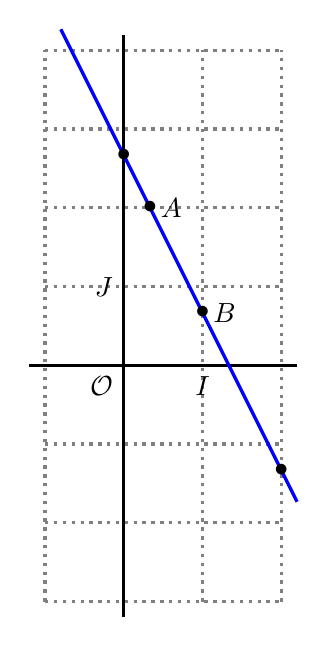
\begin{tikzpicture}[domain=-1:2,very thick]
      \draw[dotted,color=gray] (-1,-3) grid (2,4);
      \draw[] (-1.2,0) -- (2.2,0);
      \draw[] (0,-3.2) -- (0,4.2);

      \draw (0,0) node[below left]{$\mathcal{O}$};
      \draw (1,0) node[below]{$I$};
      \draw (0,1) node[left]{$J$};

      \draw[domain=-0.8:2.2,smooth,blue] plot ({\x},{-2*\x+8/3});
      \draw (0, {8/3}) node{$\bullet$};
      \draw (2, {-4/3}) node{$\bullet$};
      \draw ({1/3}, 2) node{$\bullet$} node[right]{$A$};
      \draw (1, {2/3}) node{$\bullet$} node[right]{$B$};

    \end{tikzpicture}

    On observe :
    \begin{itemize}
      \item le coefficient directeur est bien -2 (si l'on se déplace d'une unité sur l'axe des abscisses, on descend de deux unités sur l'axe des ordonnées) ;
      \item l'ordonnée à l'origine est bien $\frac{8}{3}$ ;
      \item la fonction est bien : positive avant $\frac{4}{3}$, négative après ;
      \item les points $A$ et $B$ appartiennent bien à la droite.
    \end{itemize}
  \end{multicols}
  \end{enumerate}
\end{exercice}

\begin{exercice}[Tableau de signe]~

  \emph{Tracer la courbe d'une fonction (pas nécessairement affine) qui puisse correspondre au tableau de signes suivant.}

      \begin{center}
        \begin{tikzpicture}
          \tkzTabInit[lgt=2,espcl=2]
          {$x$ /1,
            $f(x)$ /1
          }
          {$-2$,$3$, $5$, $10$, $12$}%
          \tkzTabLine{, -, z ,+ ,z,-,z,+}
        \end{tikzpicture}
      \end{center}

      Voici un exemple (parmi d'autres).
      \begin{center}
    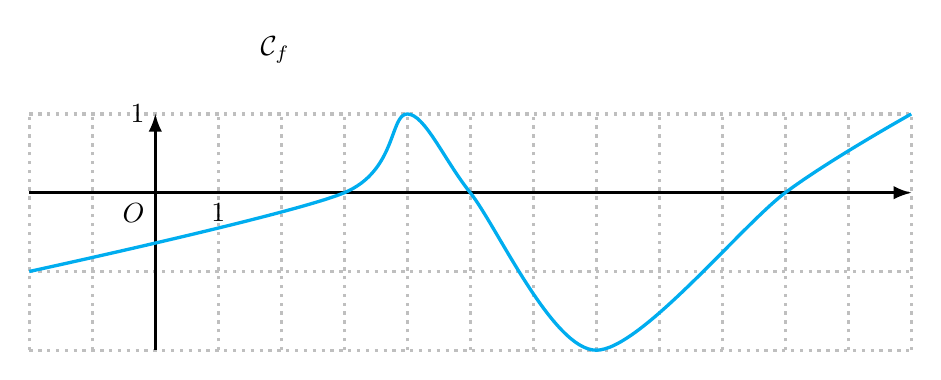
\begin{tikzpicture}[very thick,xscale=0.8, yscale=1]
      \draw[dotted, lightgray, xstep=1, ystep=1] (-2, -2) grid (12, 1);
      \draw[-latex] (-2,0) -- (12,0);
      \draw[-latex] (0,-2) -- (0,1);
      \draw (0, 1) node[left]{$1$};
      \draw (1, 0) node[below]{$1$};
      \draw [cyan] plot [smooth, tension=0.5] coordinates {
        (-2, -1)
        (3, 0)
        (4, 1)
        (5, 0)
        (7, -2)
        (10, 0)
        (12, 1)
      };
      \draw (0,0) node[below left]{$O$};
      \draw (1.5, 1.5) node[above right]{$\mathcal{C}_f$};
    \end{tikzpicture}
  \end{center}
\end{exercice}

\pagebreak

\begin{exercice}[Vecteurs]
  \emph{Soient $ABCD$ un quadrilatère quelconque, et $I$, $J$, $K$, $L$ les milieux respectifs de $[AB]$, $\left[ BC \right]$, $\left[ CD \right]$ et $\left[ DA \right]$.}

  \begin{enumerate}
    \item \emph{Faire une figure.}
      \begin{center}
        \begin{tikzpicture}[xscale=2]
          \coordinate (A) at (1, 1);
          \coordinate (B) at (1, 2);
          \coordinate (C) at (2, 2);
          \coordinate (D) at (4, 0);
          \coordinate (I) at ($.5*(A)+.5*(B)$);
          \coordinate (J) at ($.5*(B)+.5*(C)$);
          \coordinate (K) at ($.5*(C)+.5*(D)$);
          \coordinate (L) at ($.5*(D)+.5*(A)$);
          \draw (A) node[below left]{$A$};
          \draw (B) node[above left]{$B$};
          \draw (C) node[above right]{$C$};
          \draw (D) node[below right]{$D$};
          \draw (I) node{$\times$} node[left]{$I$};
          \draw (J) node{$\times$} node[above]{$J$};
          \draw (K) node{$\times$} node[right]{$K$};
          \draw (L) node{$\times$} node[below]{$L$};
          \draw (A) -- (B) -- (C) -- (D) -- cycle;
          \draw[dashed] (I) -- (J) -- (K) -- (L) -- cycle;
        \end{tikzpicture}
      \end{center}
    \item \emph{À l'aide (entre autres) de la relation de Chasles, montrer que $\vecteur{IJ}=\frac{1}{2}\vecteur{AC}$.}
      \begin{multicols}{2}
      Puisque $I$ est le milieu de $\left[ AB \right]$, alors $2\vecteur{IB}=\vecteur{AB}$. De même, $2\vecteur{BJ}=\vecteur{BC}$. Donc :

      \begin{align*}
      \vecteur{IJ} &= \vecteur{IB}+\vecteur{BJ} \\
      &= \frac{1}{2}\vecteur{AB} + \frac{1}{2}\vecteur{BC}\\
      &= \frac{1}{2}\left( \vecteur{AB}+\vecteur{BC} \right)\\
      &=\frac{1}{2}\vecteur{AC}
      \end{align*}
    \end{multicols}
    \item 
      \emph{De même, montrer que $\vecteur{LK}=\frac{1}{2}\vecteur{AC}$.}
      \begin{multicols}{2}
      De même, $2\vecteur{LD}=\vecteur{AD}$ et $2\vecteur{DK}=\vecteur{DC}$. Donc :

      \begin{align*}
      \vecteur{LK} &= \vecteur{DK}+\vecteur{LD} \\
      &= \frac{1}{2}\vecteur{DC} + \frac{1}{2}\vecteur{AD}\\
      &= \frac{1}{2}\left( \vecteur{DC}+\vecteur{AD} \right)\\
      &=\frac{1}{2}\vecteur{AC}
      \end{align*}
    \end{multicols}
    \item \emph{En déduire la nature du quadrilatère $IJKL$.}
      Nous avons montré que $\vecteur{IJ}=\frac{1}{2}\vecteur{AC}=\vecteur{LK}$, donc $\vecteur{IJ}=\vecteur{LK}$ et $IJKL$ est un parallélogramme.
    \item \emph{Quelle propriété du collège venez-vous de démontrer ?} Nous venons de démontrer que le quadrilatère formé par les milieux des quatres côtés d'un quadrilatère quelconque est un parallélogramme.
  \end{enumerate}
  

\end{exercice}

\end{document}
